\chapter{Analisi e validazione dei risultati}
\label{analisi}

\section{Analisi temporale}
\label{analisiTemporale}
Questo tipo di analisi è stata effettuata al fine di determinare la frequenza massima entro la quale il microcontrollore è in grado di eseguire tutte le operazioni basilari, rappresentate in Fig.\ref{fig:op}. Ovvero per rispondere alla seguente domanda:
\begin{quotation}
	\textit{Qual'è la finestra temporale minima sufficiente a garantire 
		che il microcontrollore sia in grado di eseguire correttamente le funzioni basilari? }
\end{quotation}
Dove per funzioni basilari si intendono le operazioni di:
\begin{itemize}
	\item \textbf{Lettura} dei dati grezzi dall'IMU tramite, indicato con $T_{RX\_I2C}$
	\item \textbf{Elaborazione} dei dati grezzi (solo per le modalità \textit{HCM} e \textit{TCM}), indicato con $T_{MotionFX}$
	\item \textbf{Trasmissione} dei dati verso il modulo \textit{App} (si veda\ref{livello_moduli}), indicato con $T_{TX\_USB}$
\end{itemize}


\begin{figure}[H]
	\centering
	\label{fig:op}    
	\subfigure[]{\label{fig:op1}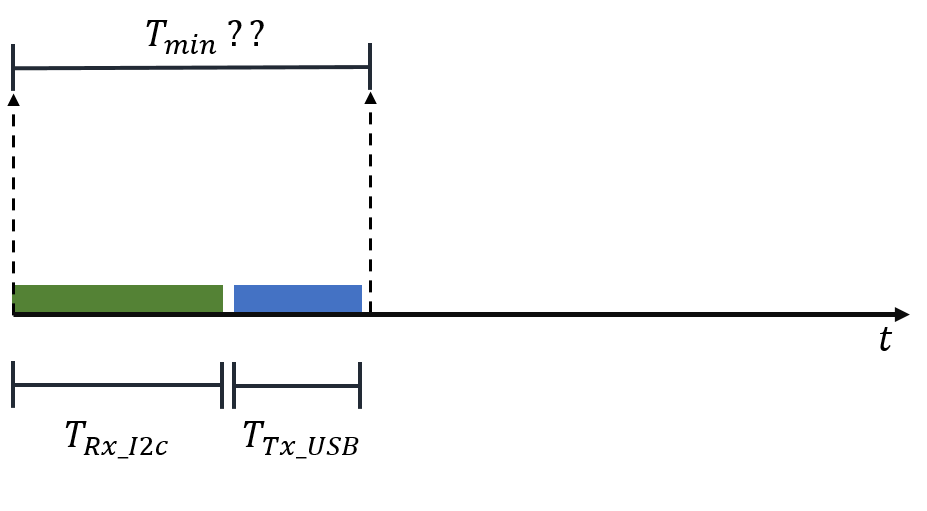
\includegraphics[width=60mm]{analisi/op1.png}}
	\subfigure[]{\label{fig:op2}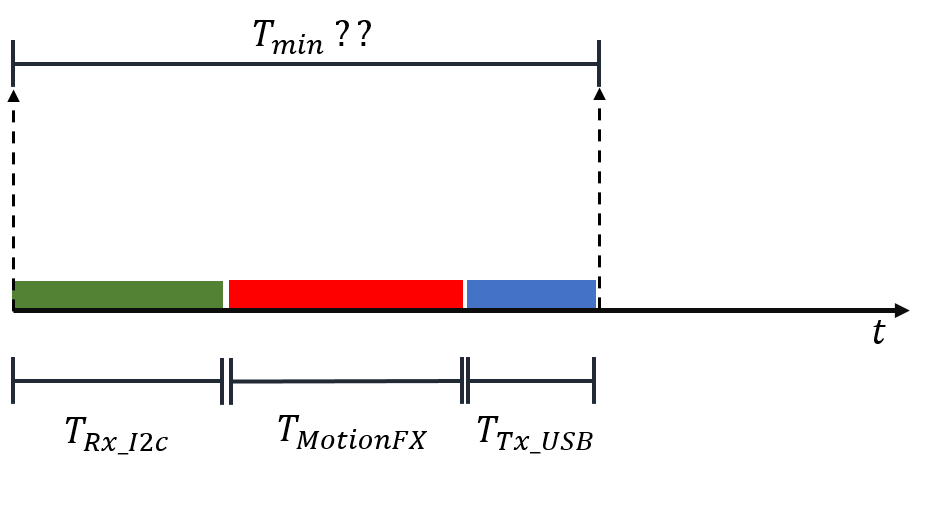
\includegraphics[width=60mm]{analisi/op2.png}}
	\caption{In \ref{fig:op1} le operazioni basilari per la modalità \textbf{LCM}, in \ref{fig:op2} le operazioni basilari per le modalità \textbf{HCM} e \textbf{TCM}}
\end{figure}

Per far ciò è opportuno analizzare singolarmente i due tempi, considerando le relative informazioni e la velocità del mezzo di comunicazione.\\

\subsection{Analisi del tempo di lettura dei dati grezzi dall'IMU}
\label{analisii2c}
Le informazioni riguardanti le grandezze fisiche misurate dai sensori integrati nell'IMU (Cap.\ref{tecnologie}), tramite I2C (Cap.\ref{imp_i2c}), su un singolo asse del \textit{b-frame} (Cap.\ref{modello_di_misura}), sono rappresentate attraverso \textbf{16 bit}.\\
Di conseguenza il tempo di lettura $T_{RX\_I2C}$ è dato dalla seguene equazione:
\begin{equation}
\label{eq:ti2c}
	T_{RX\_I2C} = N_{sensori} \cdot N_{assi} \cdot T_{i\_asse}
\end{equation}
Dove:
\begin{itemize}
	\item $N_{sensori}$ sono il numero di sensori utilizzati 
	\item $N_{assi}$ sono il numero di assi utilizzati dai sensori
	\item $ T_{i\_asse}$ è il tempo di lettura del singolo asse
\end{itemize}

Dunque il problema si riduce alla determinazione di $ T_{i\_asse}$. Per come è implementata l'IMU, la lettura di un singolo asse si completa leggendo due registri da \textbf{8 bit}.
\begin{equation}
 T_{i\_asse} = 2 \cdot T_{RX\_8bit}
\end{equation}

Per stimare $T_{RX\_8bit}$ si è programmato il microcontrollore in modo tale da leggere 1000 volte un registro da 8 bit e misurare il tempo trascorso leggendo i \textit{tick} di sistema. Per il codice si rimanda alla lettura dell'App.\ref{app:stimai2c}.\\ 
Eseguendo il test svariate volte, si è osservato che il tempo necessario per leggere 1000 volte un registro da 8 bit è pari a $101 ms$. 
Questo implica un \textit{goodput} di $80 Kb/s$ pari al $20\%$ della capacità del canale di comunicazione, che risulta essere $400 Kb/s$ essendo un I2C in \textit{fast-mode}. Questo calo è dovuto a numerosi fattori tra i quali l'overhead del protocollo e la velocità del microcontrollore.\\
Quindi andando a sostituire il valore stimato per la lettura di 8 bit nell'Eq.\ref{eq:ti2c} si ottiene, per l'uso dell'IMU a 9DOF:
\begin{equation}
T_{RX\_I2C} = 3 \cdot 3 \cdot (2 \cdot T_{RX\_8bit}) = 3 \cdot 3 \cdot (2 \cdot 101\mu s )= 1,8 ms
\end{equation}
Mentre per l'uso a 6DOF:
\begin{equation}
T_{RX\_I2C} = 3 \cdot 2 \cdot (2 \cdot T_{RX\_8bit}) = 3 \cdot 2 \cdot (2 \cdot 101\mu s )= 1,2 ms
\end{equation}


\subsection{Analisi del tempo di trasmissione dei dati tramite USB}
\label{analisiusb}
Il tempo necessario per trasmettere un pacchetto, dal modulo \textit{microcontrollore} al modulo \textit{App} (Cap.\ref{livello_sottosistemi}) mediante il canale USB (Cap.\ref{imp_usbcdc}), è dato dalla seguente equazione:
\begin{equation}
\label{tx_usb}
T_{TX\_USB}=  \frac{dim(pack)}{goodput}
\end{equation}
Per stimare il \textit{goodput} si è programmato il microcontrollore in modo da inviare 1000 volte un pacchetto contente un \textit{id} (univoco e incrementale) e un contatore incrementato quando il buffer di trasmissione risulta essere ancora occupato. Per il codice si rimanda alla lettura dell'App.\ref{app:stimausb}.
Eseguendo il test numerose volte, si è osservato che il tempo necessario per trasmettere 1000 pacchetti, per un totale di 8574 Bytes, è di circa $57 ms$. 
Questo implica un \textit{goodput} di $1,2 Mb/s$ pari al $10\%$ della capacità del canale di comunicazione che, essendo un USB 1.1, risulta essere $12 Mb/s$. Ancora una volta questo calo di prestazioni è dovuto a numerosi fattori tra i quali l'overhead del protocollo, l'implementazione della libreria STM utilizzata e la velocità del microcontrollore.\\
Più complicato è il discorso riguardante la dimensione dei pacchetti da trasmettere, questi infatti sono strettamente correlati a:
 \begin{itemize}
 	\item \textbf{La modalità di computazione} selezionata (Cap.\ref{computationMode})
 	\item \textbf{Il numero di sensori} utilizzati
 	\item \textbf{La codifica} dell'informazione
  \end{itemize}

Con riferimento alle possibili combinazioni dei fattori precedenti e alle rispettive strutture dei pacchetti, dettagliate nel Cap.\ref{computationMode}, si hanno le seguenti dimensioni: 
\begin{enumerate}
	\item \textbf{LCM}:
		\begin{enumerate}
		\item \textit{6DOF} = 48 Bytes
		\item \textit{9DOF} = 63 Bytes
		\end{enumerate}
	\item \textbf{HCM} = 21 Bytes
	\item \textbf{TCM}:
			\begin{enumerate}
			\item \textit{6DOF} = 63 Bytes
			\item \textit{9DOF} = 84 Bytes
			\end{enumerate}
\end{enumerate}

Sostituendo questi valori e la stima del \textit{goodput} del canale all'Eq.\ref{tx_usb}, si ottengono le stime dei diversi tempi di trasmissione:

\begin{enumerate}
	\item \textbf{LCM}:
	\begin{enumerate}
		\item \textit{6DOF}: $ T_{TX\_USB}=  \frac{48 Bytes}{1,2 Mbit/s} = 0,32 ms $
		\item \textit{9DOF} : $ T_{TX\_USB}=  \frac{63 Bytes}{1,2 Mbit/s} = 0,42 ms $
	\end{enumerate}
	\item \textbf{HCM} : $ T_{TX\_USB}=  \frac{21 Bytes}{1,2 Mbit/s} = 0,16 ms $
	
	\item \textbf{TCM}:
	\begin{enumerate}
		\item \textit{6DOF} : $ T_{TX\_USB}=  \frac{63 Bytes}{1,2 Mbit/s} = 0,42 ms $
		\item \textit{9DOF} : $ T_{TX\_USB}=  \frac{84 Bytes}{1,2 Mbit/s} = 0,56 ms $
	\end{enumerate}
\end{enumerate}



\subsection{Conclusioni analisi temporale}
Sommando i tempi stimati nei paragrafi precedenti (Cap.\ref{analisii2c} e Cap.\ref{analisiusb}), si ottengono le diverse finestre temporali minime affinché, il microcontrollore riesca a completare le funzioni basilari:

\begin{enumerate}
	\item \textbf{LCM}:
	\begin{enumerate}
		\item \textit{6DOF}: $T_{min} = T_{RX\_I2C} + T_{TX\_USB} = 1,2 ms + 0,32 ms = 1,52 ms $
		\item \textit{9DOF} : $ T_{min} = T_{RX\_I2C} + T_{TX\_USB} = 1,8 ms + 0,42 ms = 2,22 ms $
	\end{enumerate}
	\item \textbf{HCM} :
		\begin{enumerate}
		\item \textit{6DOF}: $T_{min} = T_{RX\_I2C} + T_{TX\_USB} = 1,2 ms + 0,16 ms = 1,36 ms $
		\item \textit{9DOF} : $ T_{min} = T_{RX\_I2C} + T_{TX\_USB} = 1,8 ms + 0,16 ms = 1,96 ms $
	\end{enumerate}
	\item \textbf{TCM}:
	\begin{enumerate}
		\item \textit{6DOF} : $ T_{min} = T_{RX\_I2C} + T_{TX\_USB} = 1,2 ms + 0,42 ms = 1,62 ms $
		\item \textit{9DOF} : $T_{min} = T_{RX\_I2C} + T_{TX\_USB} = 1,8 ms + 0,56 ms = 2,36 ms $
	\end{enumerate}
\end{enumerate}

 Da notare che tali stime non tengono conto di alcune latenze legate all'esecuzione del codice all'interno del microprocessore, per questo motivo si ritiene opportuno sovrastimare le finestre temporali e sottostimare le frequenze massime, in modo da avere margini di sicurezza e stabilità maggiori.\\
Per le modalità \textit{HCM} e \textit{TCM} si deve tener conto anche del tempo di computazione della libreria \textit{Motion FX} per la stima della dell'assetto a partire dai dati grezzi che, nel caso peggiore è dichiarato essere $3,2 ms$ \cite{motion} per il microcontrollore utilizzato nell'ambito di questa tesi.\\
Quindi le stime aggiornate risultano essere:
\begin{enumerate}
	\item \textbf{LCM}:
	\begin{enumerate}
		\item \textit{6DOF}: $T_{min} = T_{RX\_I2C} + T_{TX\_USB} = 1,2 ms + 0,32 ms = 1,52 ms $
		\item \textit{9DOF} : $ T_{min} = T_{RX\_I2C} + T_{TX\_USB} = 1,8 ms + 0,42 ms = 2,22 ms $
	\end{enumerate}
	\item \textbf{HCM} :
	\begin{enumerate}
		\item \textit{6DOF}: $T_{min} = T_{RX\_I2C} + T_{TX\_USB} + T_{MotionFX}  = 1,2 ms + 0,16 ms + 3,2ms = 4,56 ms $
		\item \textit{9DOF} : $ T_{min} = T_{RX\_I2C} + T_{TX\_USB} + T_{MotionFX} = 1,8 ms + 0,16 ms + 3,2ms = 5,16 ms $
	\end{enumerate}
	\item \textbf{TCM}:
	\begin{enumerate}
		\item \textit{6DOF} : $ T_{min} = T_{RX\_I2C} + T_{TX\_USB} + T_{MotionFX} = 1,2 ms + 0,42 ms + 3,2ms = 4,82 ms $
		\item \textit{9DOF} : $T_{min} = T_{RX\_I2C} + T_{TX\_USB} + T_{MotionFX} = 1,8 ms + 0,56 ms + 3,2 ms = 5,56 ms $
	\end{enumerate}
\end{enumerate}

 
Che corrispondono alle seguenti frequenze di lavoro massime:

\begin{enumerate}
	\item \textbf{LCM}:
	\begin{enumerate}
		\item \textit{6DOF}: $f = 657 Hz $
		\item \textit{9DOF} : $f = 450 Hz $
	\end{enumerate}
	\item \textbf{HCM} :
	\begin{enumerate}
		\item \textit{6DOF}: $f = 219 Hz $
		\item \textit{9DOF} : $f = 193 Hz $
	\end{enumerate}
	\item \textbf{TCM}:
	\begin{enumerate}
		\item \textit{6DOF} : $f = 207 Hz $
		\item \textit{9DOF} : $f = 179 Hz $
	\end{enumerate}
\end{enumerate}

\section{Analisi dello zero-offset}
Quest'analisi è stata effettuata al fine di stimare lo \textbf{zero-offset} dell'accelerometro e del giroscopio. Tale fenomeno consiste nella deviazione dei dati in output dai sensori (\ref{imp_i2c}) rispetto al valore ideale atteso quando il sensore non subisce forze esterne. L'origine di questo errore è strettamente legata agli stress meccanici subiti dall'IMU nei processi di realizzazione.\\
Relativamente ai sopra citati sensori, si hanno le seguenti definizioni di zero-offset:
\begin{itemize}
	\item \textbf{zero-g offset}: nel caso ideale un accelerometro posto in posizione orizzontale e immobile misura \textit{0 g} sugli assi X e Y mentre \textit{1 g} sull'asse Z. Lo \textit{zero-g} è la deviazione del valore letto in uscita rispetto al valore ideale.
	\item \textbf{zero-rate offset}: nel caso ideale un giroscopio immobile misura \textit{0 dps} su tutti gli assi. Lo \textit{zero-g} è la deviazione del valore letto in uscita rispetto al valore ideale.
\end{itemize}

\subsection{Stima dello zero-g offset}
Per stimare lo zero-g offset si è posto immobile l'IMU e si sono raccolti i dati letti dall'accelerometro per un totale di due minuti. Tale procedura è stata ripetuta tre volte ponendo ogni volta l'IMU parallelo rispetto ad un'asse (Cap.\ref{modello_di_misura}), come mostrato in Fig.\ref{fig:zero-g}:
\begin{figure}[H]
	\centering    
	\label{fig:zero-g}
	\subfigure[]{\label{fig:x}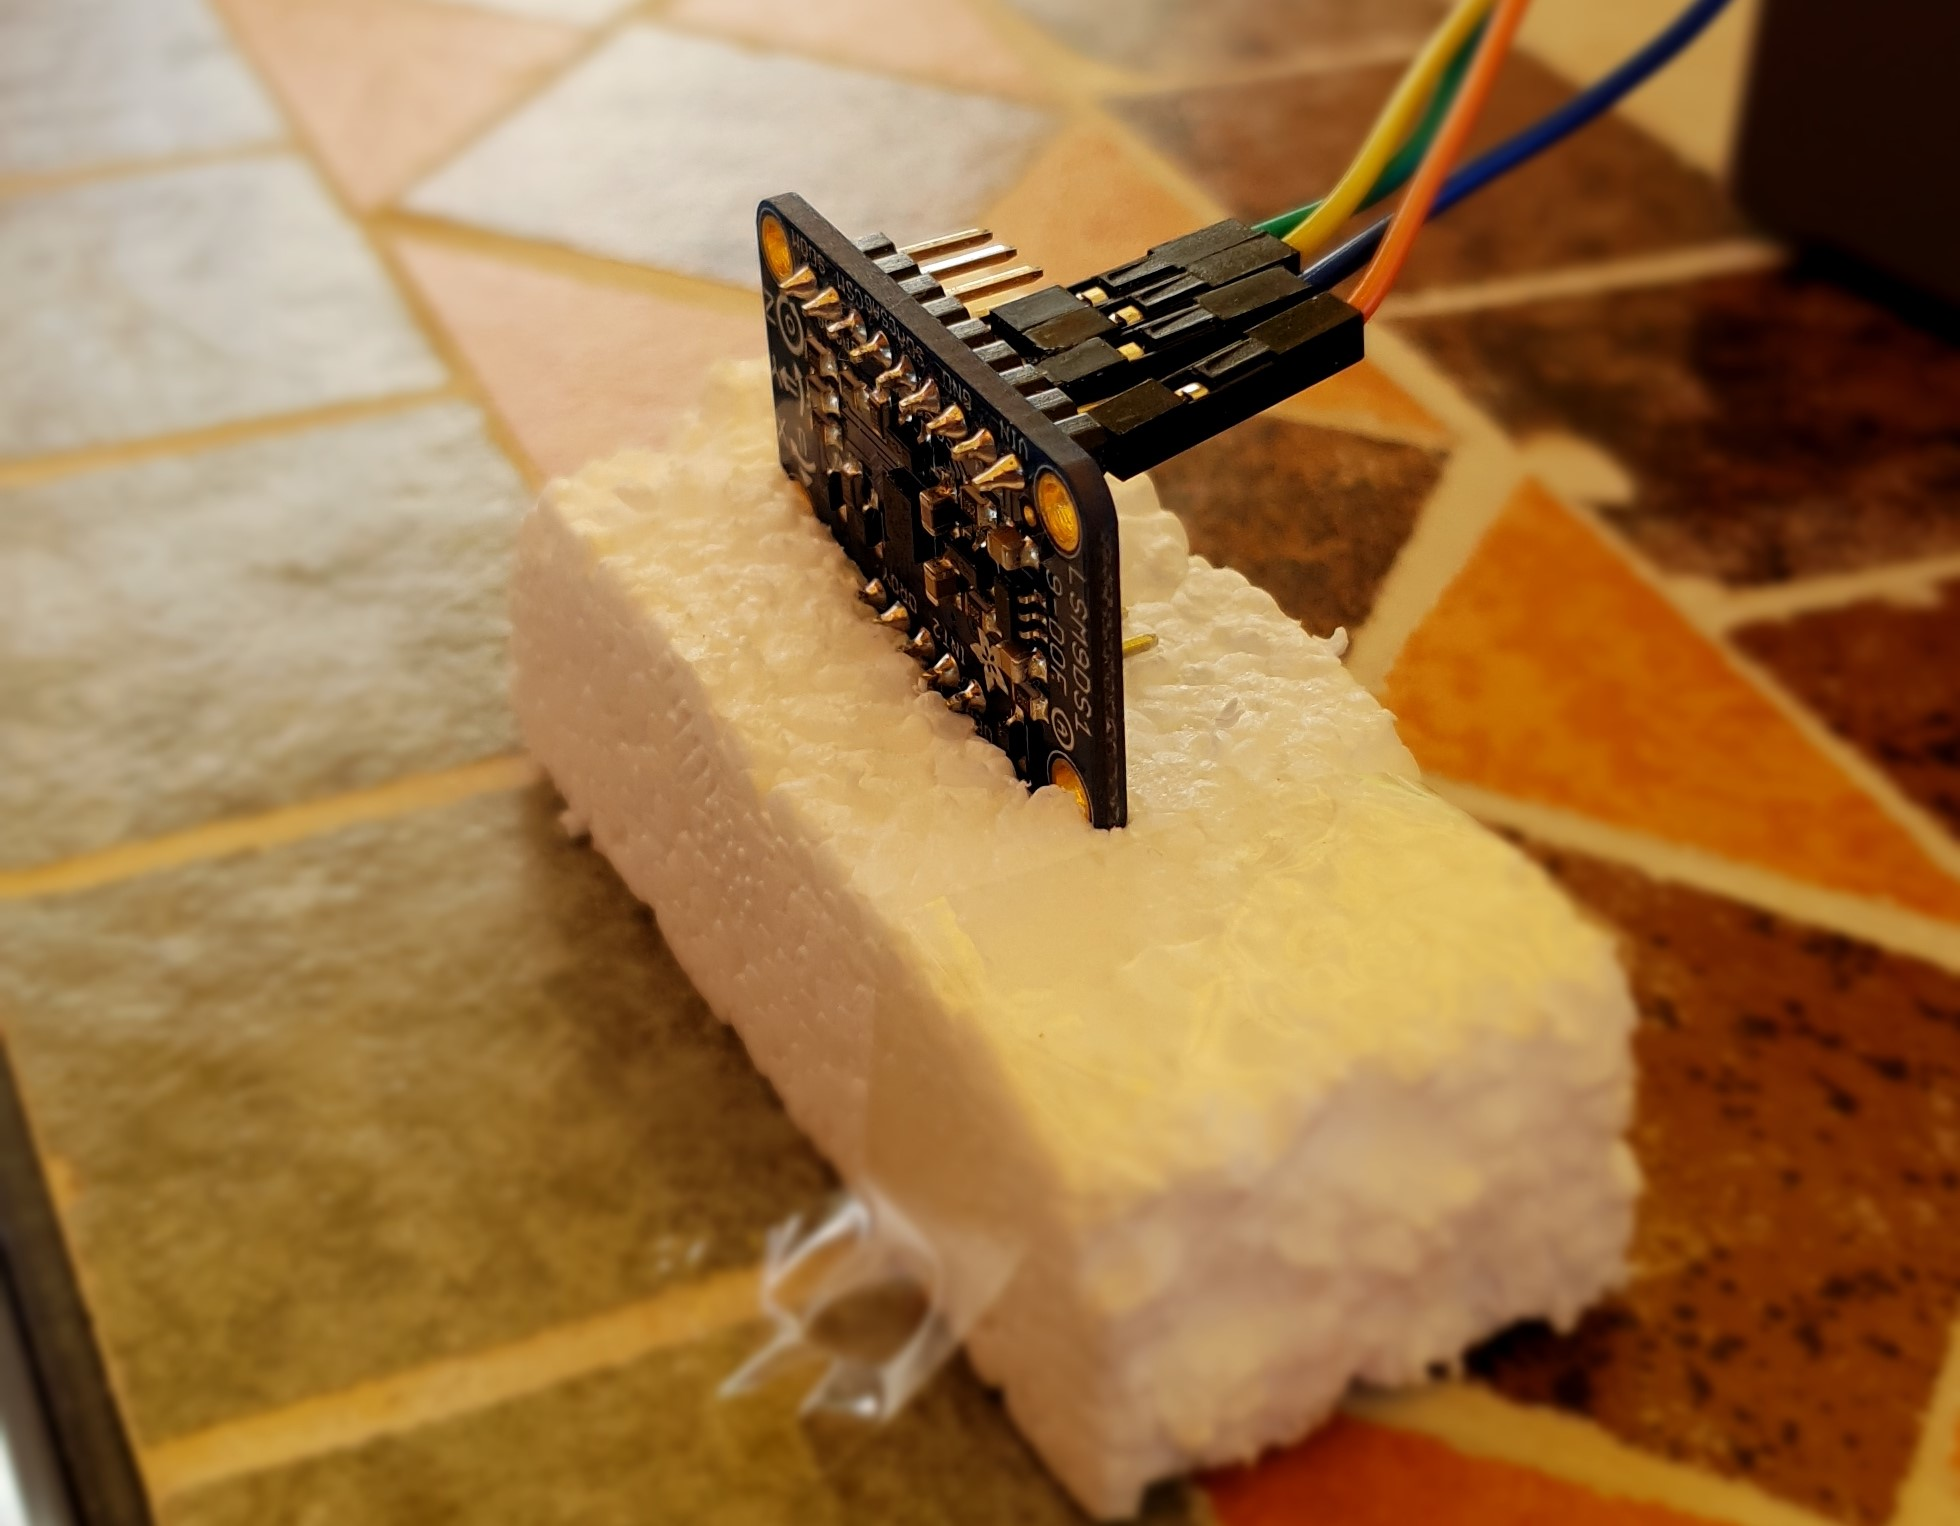
\includegraphics[width=40mm]{analisi/x.jpg}}
	\subfigure[]{\label{fig:y}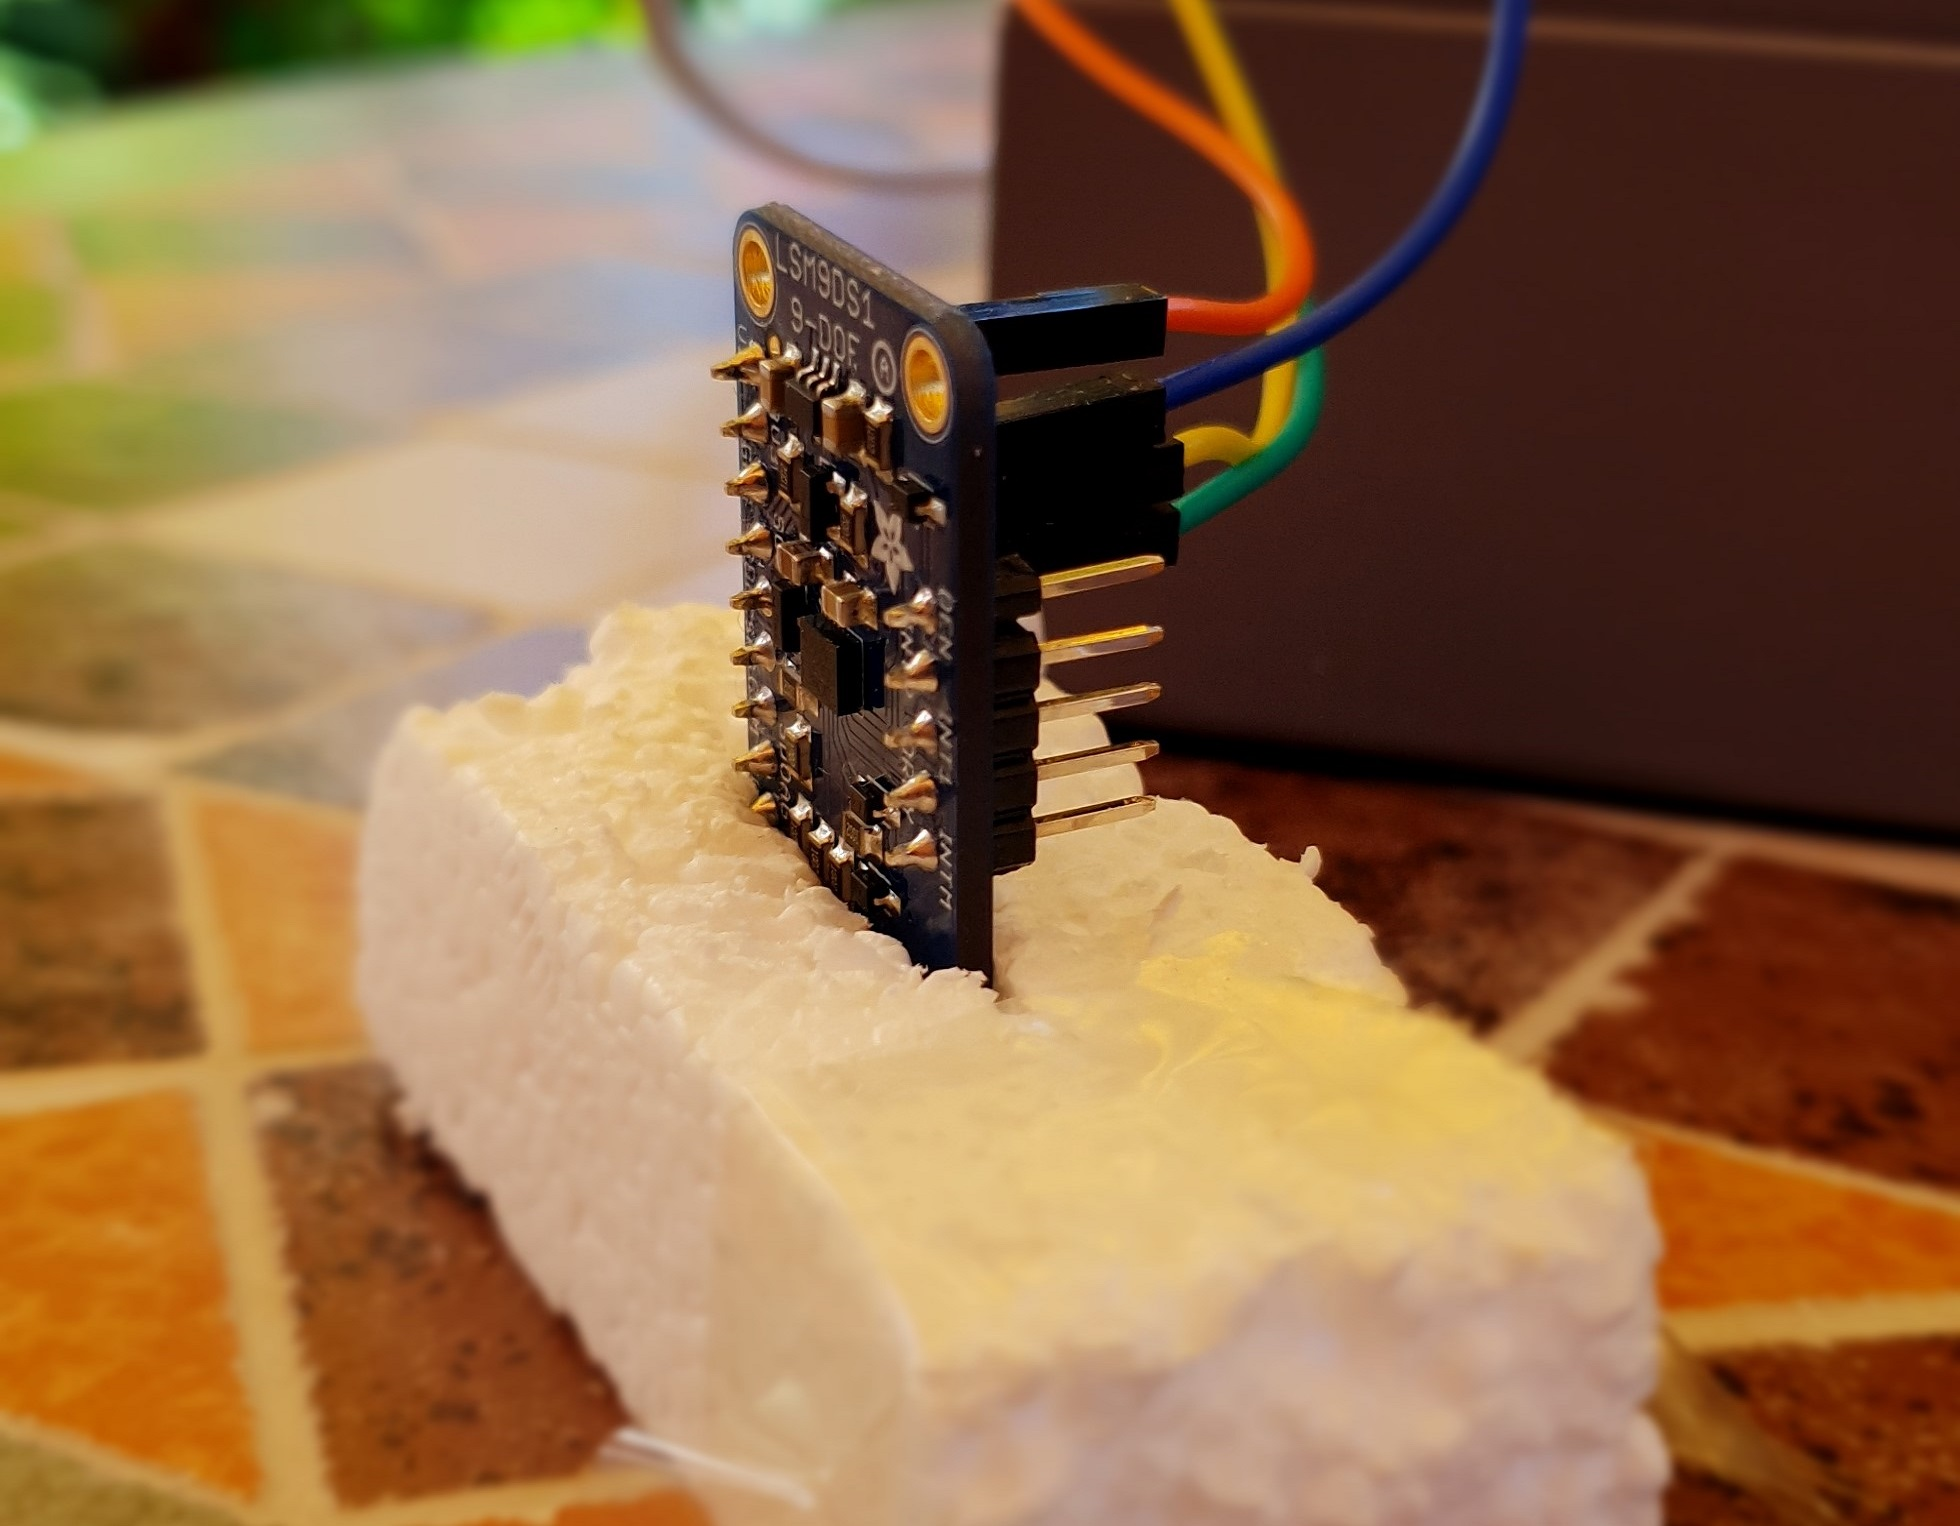
\includegraphics[width=40mm]{analisi/y.jpg}}
	\subfigure[]{\label{fig:z}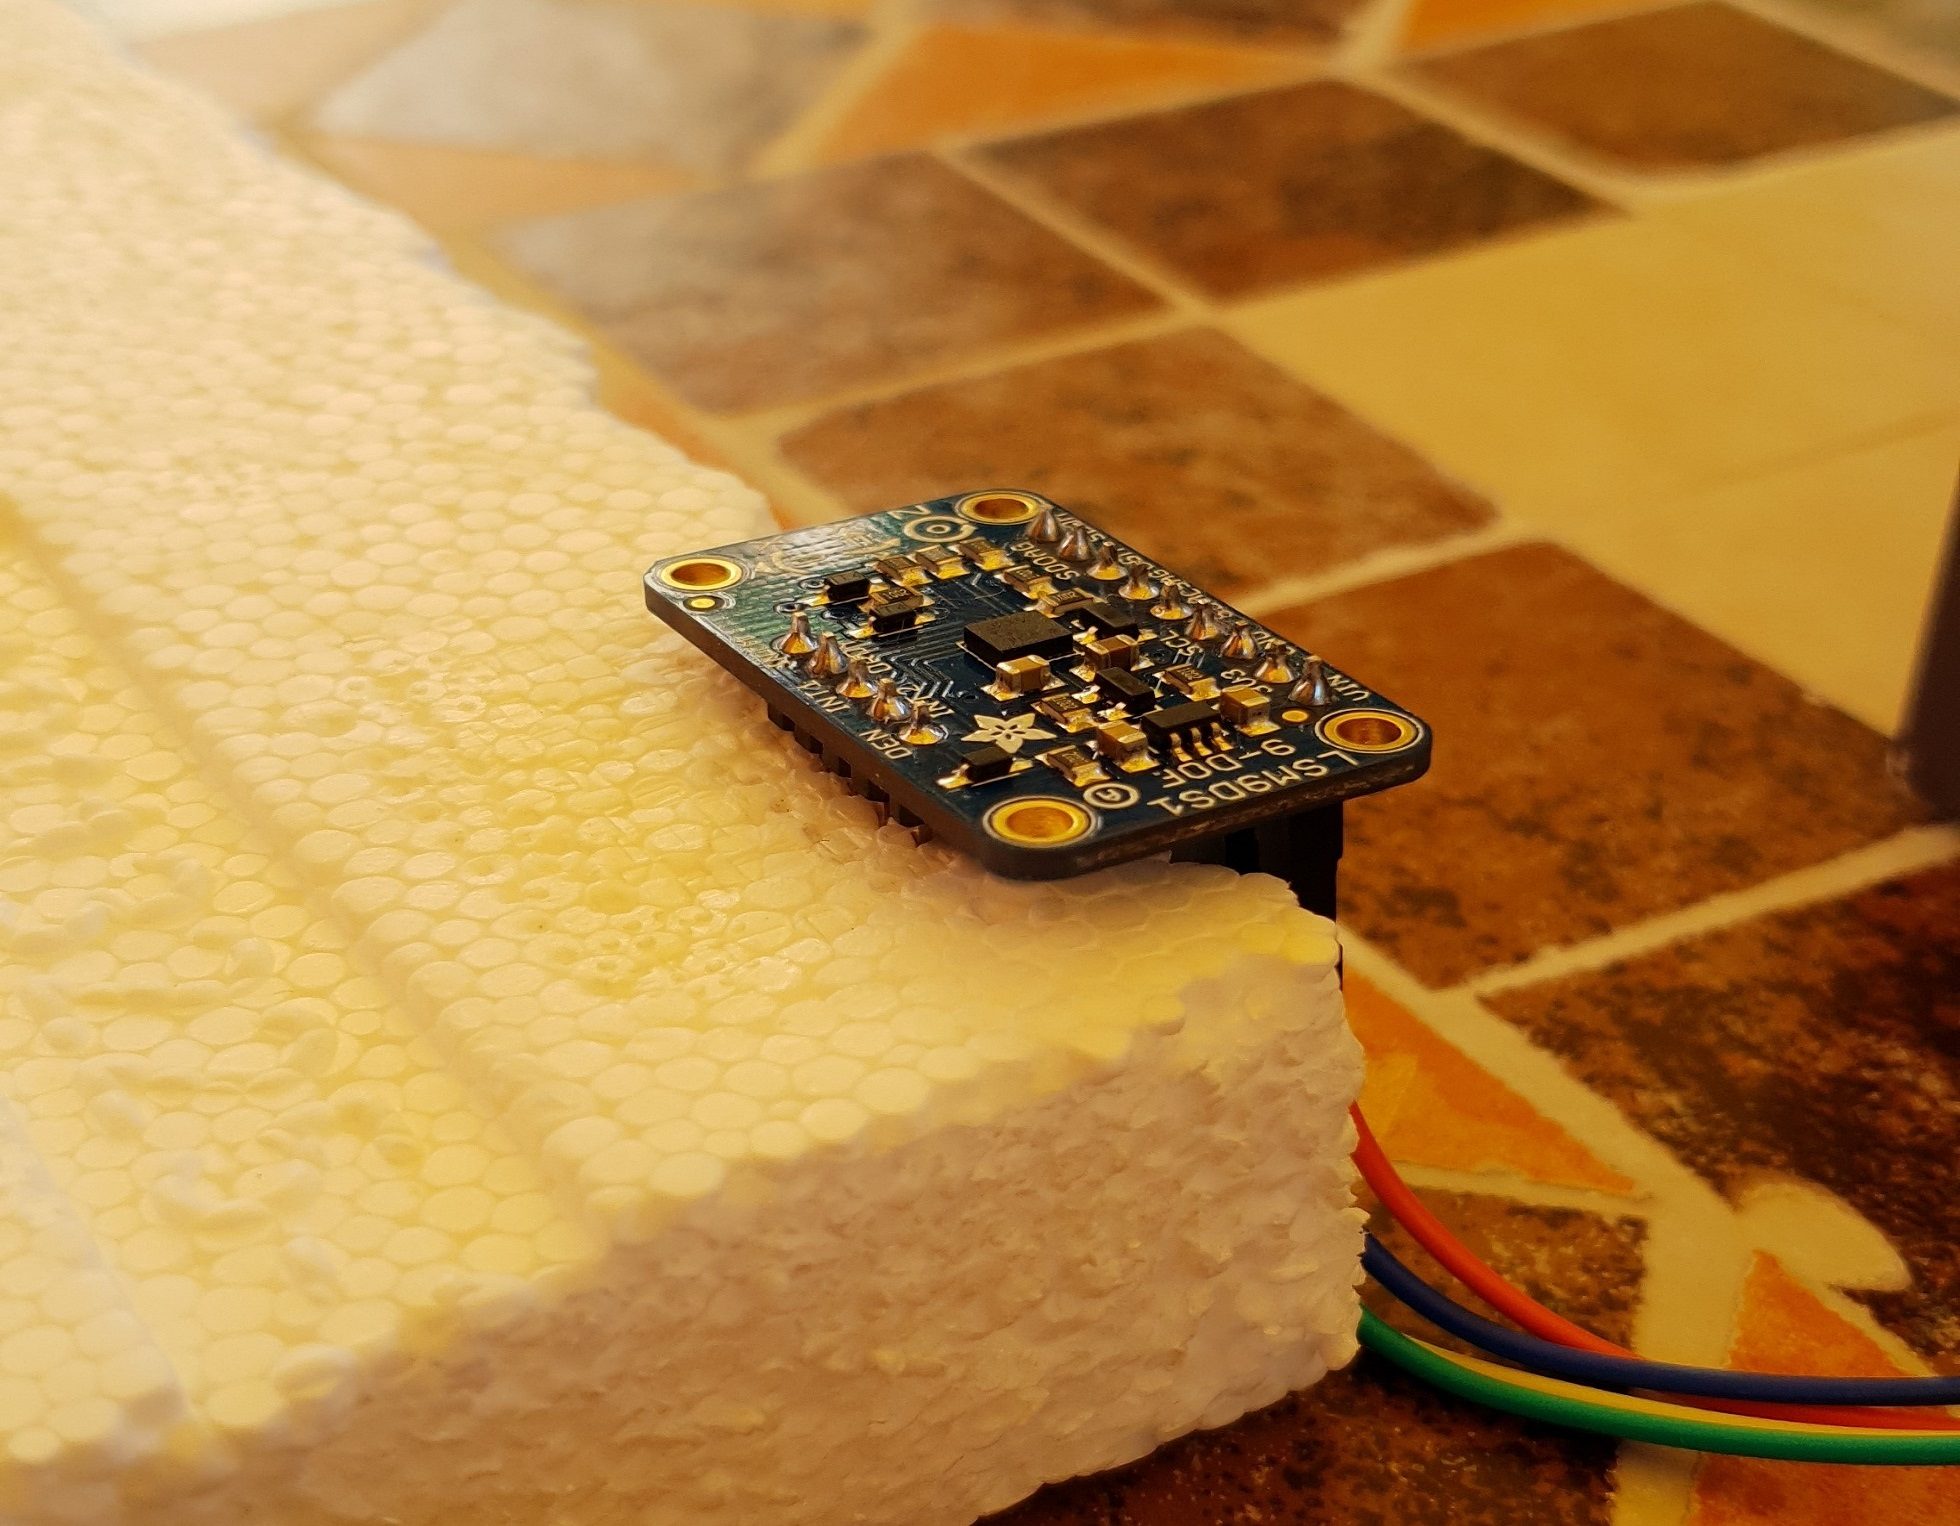
\includegraphics[width=40mm]{analisi/z.jpg}}
	\caption{in \ref{fig:x} l'IMU posto parallelamente all'asse \textit{X}, in \ref{fig:y} l'IMU posto parallelamente all'asse \textit{Y} e infine in \ref{fig:z} l'IMU posto parallelamente all'asse \textit{Z}}
\end{figure}
Quindi per ogni lettura si è determinata la norma euclidea, dalla quale banalmente si ottiene il modulo dello zero-g offset sottraendo 1. Tale valore è da considerarsi come modulo e non sui singoli assi in quanto il dispositivo potrebbe non essere stato posizionato perfettamente parallelo all'asse in questione. In Fig.\ref{fig:andamentizero-g} vengono mostrati i valori degli zero-offset per i campioni catturati nei primi 7 secondi per ognuno dei tre assi:

\begin{figure}[H]
	\centering    
	\subfigure[]{\label{fig:zgx}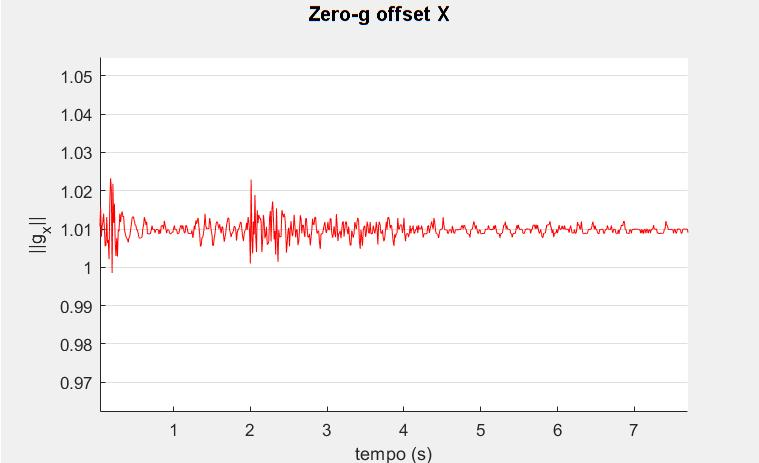
\includegraphics[width=80mm]{analisi/x-offset.jpg}}
	\subfigure[]{\label{fig:zgy}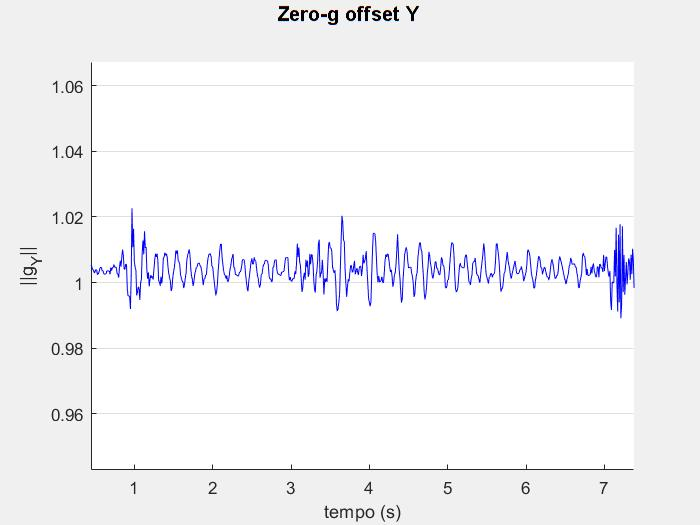
\includegraphics[width=80mm]{analisi/y-offset.jpg}}
	\subfigure[]{\label{fig:zgz}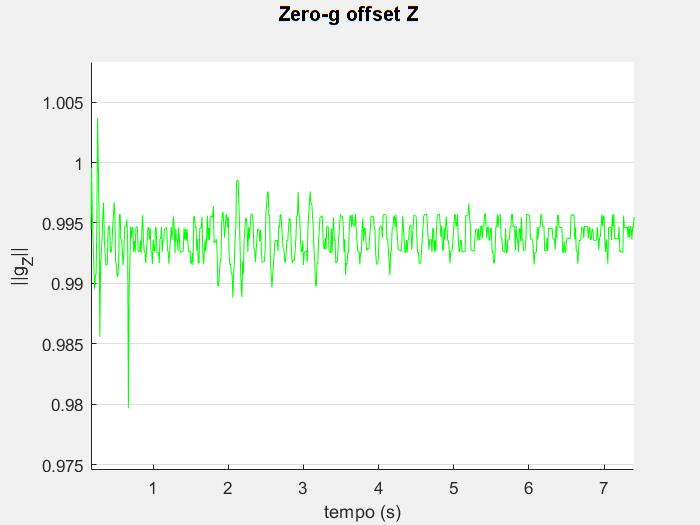
\includegraphics[width=80mm]{analisi/z-offset.jpg}}
	\label{fig:andamentizero-g}
	\caption{valori degli zero-g offset calcolati rispettivamente sull'asse X \ref{fig:zgx}, sull'asse Y  \ref{fig:zgy} e sull'asse \ref{fig:zgz}}
\end{figure}

Nella Tab.\ref{tab:zero-g} si riportano i valori di \textit{Media, Max} e le percentuali di occorrenze dei valori compresi nell'intervallo (0,1) e maggiori di 1.

\begin{table}[H]
	\centering
	\label{tab:zero-g}
	\begin{tabular}{|c|c|c|c|c|}
		\hline
		\textbf{Asse} & \multicolumn{1}{l|}{\textbf{Media (G)}} & \multicolumn{1}{l|}{\textbf{Max (G)}} & \textbf{ val>1} & \textbf{ 0<val>1} \\ \hline
			x             & 1,0096                                  & 1,0233                                & 99               & 1                  \\ \hline
			y             & 1,0036                                  & 1,0266                                & 99               & 1                  \\ \hline
			z             & 0,9936                                  & 1,0037                                & 0,02             & 99,08              \\ \hline
		\end{tabular}
	\caption{Media, Max e percentuali di occorrenze dei valori compresi nell'intervallo (0,1) e maggiori di 1 dei dati mostrati in Fig.\ref{fig:zgx} }
	\end{table}


\subsection{Stima dello zero-rate offset}
Per stimare lo zero-rate offset si è posto immobile l'IMU (come in Fig.\ref{fig:zero-g}) e si sono raccolti i dati letti dal giroscopio per un totale di due minuti. I valori ottenuti, per ognuno dei tre assi, sono mostrati in Fig.\ref{fig:zero-rate}:
\begin{figure}[H]  
	\centering 
	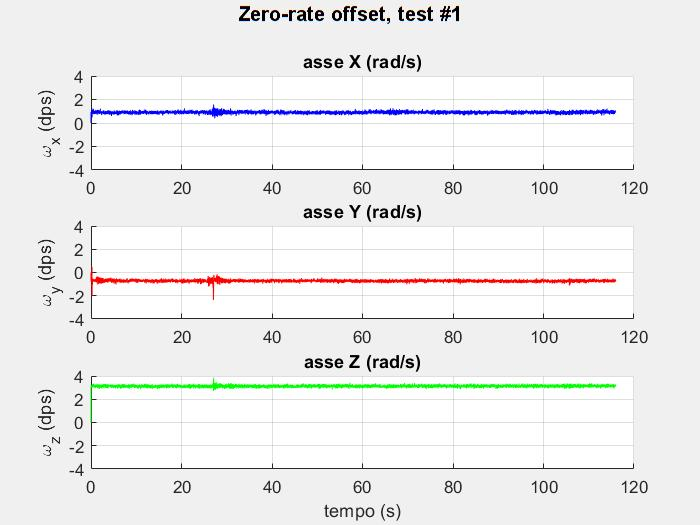
\includegraphics[scale=0.6]{analisi/zero-rate.jpg}
	\caption{valori degli zero-rate offset per i campioni catturati in 2 minuti rispettivamente sull'asse X, Y e Z.}
	\label{fig:zero-rate}
\end{figure}
Dai valori mostrati in Fig.\ref{fig:zero-rate} si evince facilmente la presenza di un offset significativo sull'asse Z da cui ne consegue che, pur rimanendo immobile il giroscopio ha \textit{"la sensazione"} di essere ruotato intorno all'asse in questione con una velocità angolare significativa.\\
Nella Tab.\ref{tab:zero-rate} si riportano invece i valori di \textit{media} e \textit{varianza} per i campioni mostrati in Fig.\ref{fig:zero-rate}:
\begin{table}[H]
	\centering
	\label{tab:zero-rate}
	\begin{tabular}{|c|c|c|l}
		\cline{1-3}
		\textbf{Asse} & \multicolumn{1}{l|}{\textbf{Media (dps)}} & \multicolumn{1}{l|}{\textbf{Varianza}} &  \\ \cline{1-3}
		x             & 0,9055                                    & 0,0079                                 &  \\ \cline{1-3}
		y             & -0,7203                                   & 0,0091                                 &  \\ \cline{1-3}
		z             & 3,1291                                    & 0,0064                                 &  \\ \cline{1-3}
	\end{tabular}
	\caption{Media e varianza per i valori di zero-rate offset mostrati in Fig.\ref{fig:zero-rate}}
\end{table}
\subsection{Conclusioni stima dello zero-offset}
L'analisi appena effettuata ha mostrato come i dati grezzi provenienti dall'unità di misura inerziale (Cap.\ref{tecnologie}) siano affetti dallo zero-offset.\\
L'accelerometro non risulta subire molto questo fenomeno, infatti i valori medi dei moduli del vettore gravitazionale si discostano al più dello 0,96\% (\ref{tab:zero-g}) sull'asse delle \textit{X} e il valore massimo si ha in corrispondenza dell'asse \textit{Y} che supera il valore ideale di $0,0266 G$. \\
Ben diversa è la situazione dello zero-rate offset che risulta essere molto significativo sopratutto sull'asse \textit{Z} dove si ha una media di $3,1291 dps$. I valori di varianza bassi sottolineano come tale errore sia relativamente constante nel tempo fornendo quindi un punto di partenza per una sua modellizzazione.\\
A valle di queste considerazioni si vuole evidenziare come l'uso dei dati grezzi provenienti dall'IMU per un'elaborazione che permetta la stima dell'assetto, debba essere preceduto da un'attività di compensazione di tali offset. Compensazione che può, in alcuni casi, trasformarsi in un vero e proprio lavoro di caratterizzazione e modellizzazione dell'errore all'interno dell'algoritmo di elaborazione. 





\section{Analisi qualitativa dell'assetto stimato}



